\documentclass{article}

\usepackage{enumerate}
\usepackage{amssymb}
\usepackage{amsmath}
\usepackage{algorithm}
\usepackage[noend]{algpseudocode}
\usepackage{graphicx}
\usepackage{listings}

\graphicspath{ {Images/} }

\topmargin=-0.45in
\evensidemargin=0in
\oddsidemargin=0in
\textwidth=6.5in
\textheight=9.0in
\headsep=0.25in

\title{CS 189: Homework 1}
\author{Michael Stephen Chen\\ Kaggle Acct: michaelstchen \\SID: 23567341}

\begin{document}
\maketitle

\pagebreak

\section*{Problem 1}
\begin{center}
$\begin{array}{cc}
  Num Imgs & Error Rate \\
  100      & 0.6858     \\
  200      & 0.7690     \\
  500      & 0.8032     \\
  1000     & 0.8353     \\
  2000     & 0.8505     \\
  5000     & 0.8701     \\
  10000    & 0.8692
\end{array}$


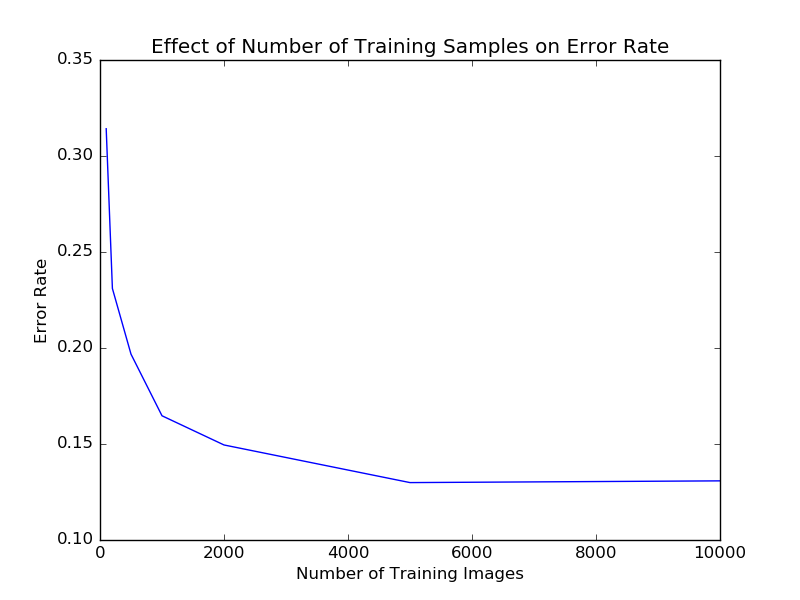
\includegraphics[scale=0.5]{errplot}
\end{center}


\section*{Problem 2}
\begin{center}
  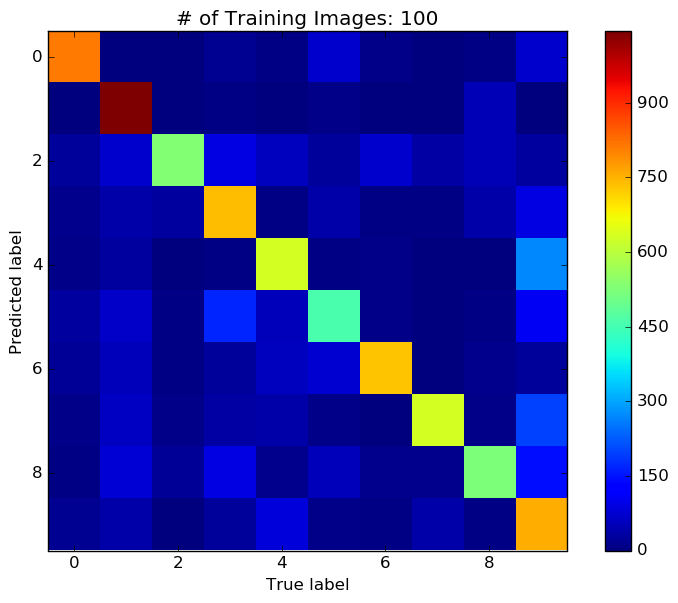
\includegraphics[scale=0.4]{100}
  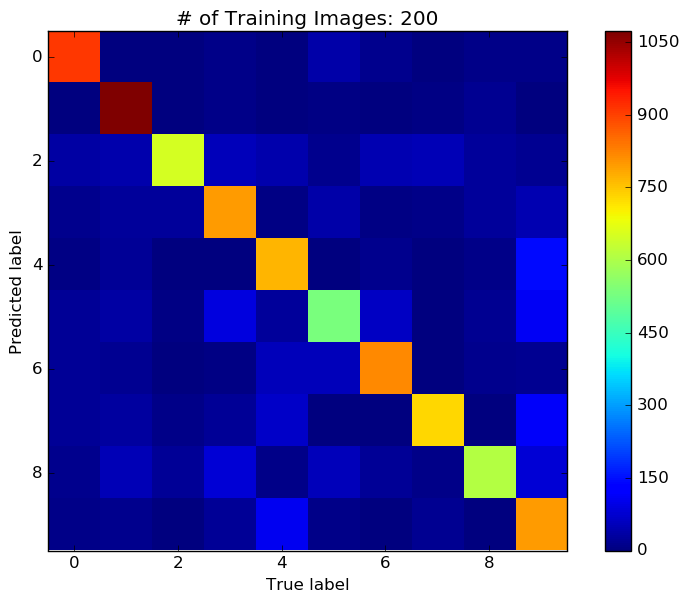
\includegraphics[scale=0.4]{200}\\
  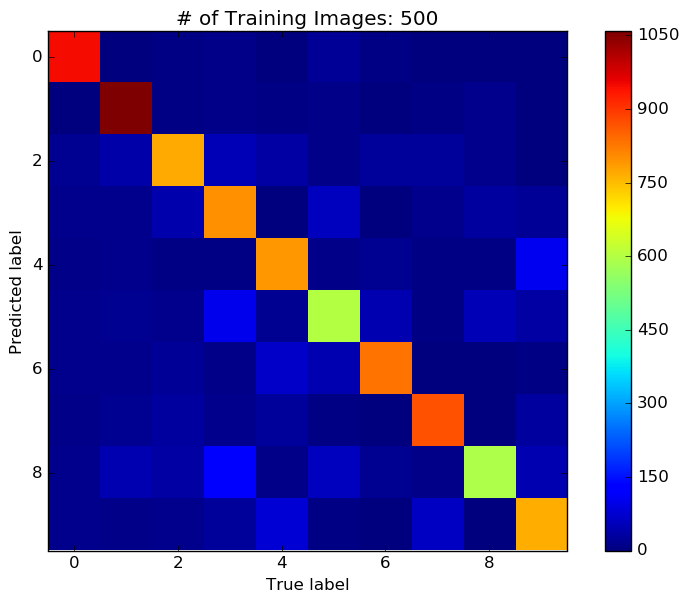
\includegraphics[scale=0.4]{500}
  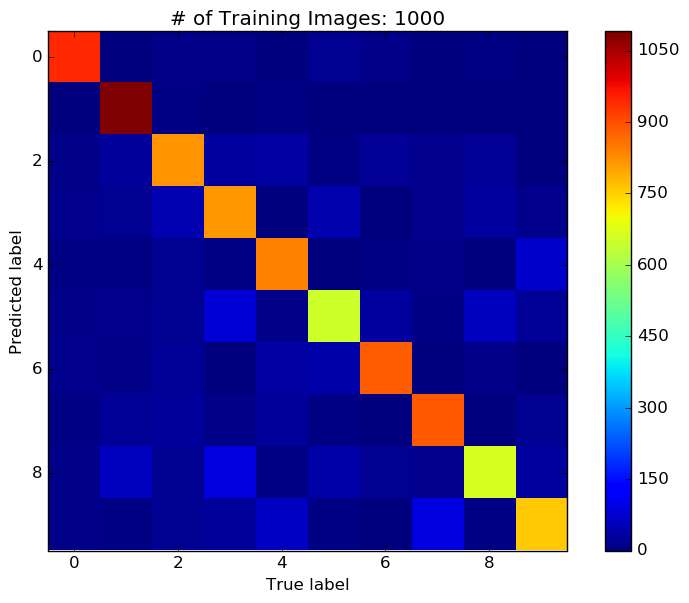
\includegraphics[scale=0.4]{1000}\\
  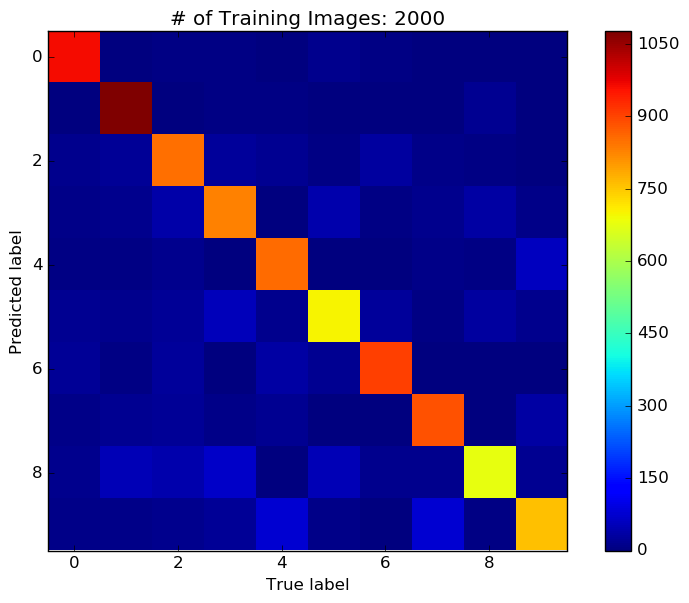
\includegraphics[scale=0.4]{2000}
  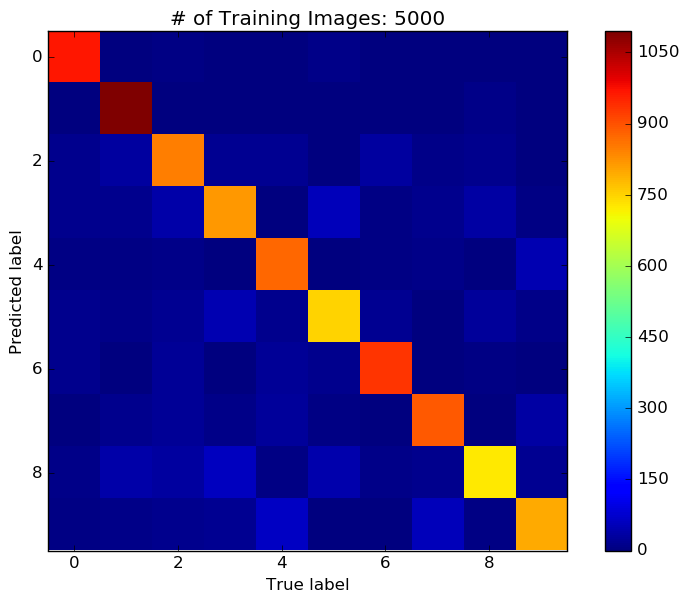
\includegraphics[scale=0.4]{5000}\\
  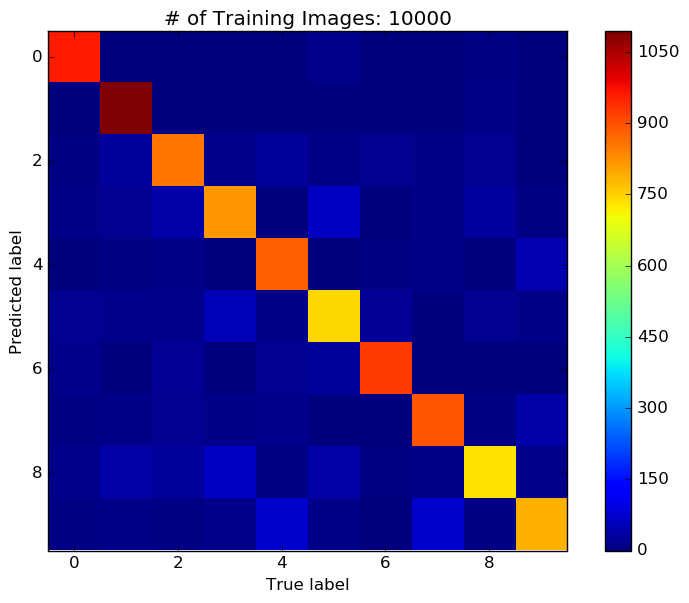
\includegraphics[scale=0.4]{10000}
\end{center}

From the confusion matrices we see that as we increase the number of training images the diagonals become "redder", indicating that our prediction accuracy is increasing, while the off-diagonals get "bluer," indicating that our error rates are going down. Both of these indicate that the accuracy of our classification method generally increases with the number of training samples.


We also see that from 2000 images onward, the change in coloring is just about unnoticeable. This is in accord with our plot from Problem 1 above that shows the error rate decreasing with an almost aymptotic character. So our naive classification method can only get us so far no matter how many training samples we use.


\section*{Problem 3}
\begin{itemize}
\item Cross-validation produces a more stable result with lower variablity because we are taking an average of $k$ trials. It also help to reduce overfitting because we don't use just one set of validation and training sets. 
\item I ran various C values during my experimental runs but I failed to record those. But I used those runs to narrow down the optimal C value. Note that I am reporting the accuracy and the error rate is just $1-accuracy$. My optimal C value was $1e-06$ with a accuracy of $0.9059$.
  \begin{center}
    $\begin{array}{cc}
       C              & Accuracy       \\
       1e-07          & 0.8962         \\
       \textbf{1e-06} & \textbf{0.9059}\\
       1e-05          & 0.8807         \\
    \end{array}$
  \end{center}
  
\item My best Kaggle score was \textbf{0.91380}.
  \item I did not modify any features.
\end{itemize}


\section*{Problem 4}
\begin{itemize}
  \item I ran 10 different C values. One thing to note is that my validation accuracies are considerably higher than my Kaggle score which may be indicative of overfitting. Also one interesting thing is that using LinearSVC instead SVC jumped my accuracy from 0.7399 to 0.79024. Again I am reporting accuracies (so $1- errorRate$). My optimal C value was 1 with a validation accuracy of 0.94023.
  \begin{center}
    $\begin{array}{cc}
       C        & Accuracy  \\
       1e-05    & 0.82640   \\
       0.0001   & 0.83897   \\
       0.001    & 0.85444         \\
       0.01     & 0.87940       \\
       0.1      & 0.93404        \\
       \textbf{1} & \textbf{0.94023} \\
       10       & 0.92708        \\
       100      & 0.92766        \\
       1000     & 0.84681        \\
       10000    & 0.87447        \\
    \end{array}$
  \end{center}

\item My best Kaggle score was \textbf{0.79024}.
  \item I added a couple more word-count features for words that I commonly saw when I was reading over the spam files (e.g. 'viagra', 'microsoft', 'www', 'sexual', etc.). Please see 'featurize.py' for more.
\end{itemize}

\pagebreak
\section*{Appendix A: prob1.py}
\lstinputlisting{prob1.py}
\pagebreak
\section*{Appendix B: prob2.py}
\lstinputlisting{prob2.py}
\pagebreak
\section*{Appendix C: prob3.py}
\lstinputlisting{prob3.py}
\pagebreak
\section*{Appendix D: prob4.py}
\lstinputlisting{prob4.py}
\pagebreak
\section*{Appendix E: featurize.py}
\lstinputlisting{featurize.py}
\end{document}
